%% (Master) Thesis template
% Template version used: v1.4
%
% Largely adapted from Adrian Nievergelt's template for the ADPS
% (lecture notes) project.


%% We use the memoir class because it offers a many easy to use features.
\documentclass[11pt,a4paper,titlepage]{memoir}

%% Packages
%% ========

%% LaTeX Font encoding -- DO NOT CHANGE
\usepackage[OT1]{fontenc}

%% Babel provides support for languages.  'english' uses British
%% English hyphenation and text snippets like "Figure" and
%% "Theorem". Use the option 'ngerman' if your document is in German.
%% Use 'american' for American English.  Note that if you change this,
%% the next LaTeX run may show spurious errors.  Simply run it again.
%% If they persist, remove the .aux file and try again.
\usepackage[english]{babel}

%% Input encoding 'utf8'. In some cases you might need 'utf8x' for
%% extra symbols. Not all editors, especially on Windows, are UTF-8
%% capable, so you may want to use 'latin1' instead.
\usepackage[utf8]{inputenc}

%% This changes default fonts for both text and math mode to use Herman Zapfs
%% excellent Palatino font.  Do not change this.
\usepackage[sc]{mathpazo}

%% The AMS-LaTeX extensions for mathematical typesetting.  Do not
%% remove.
\usepackage{amsmath,amssymb,amsfonts,mathrsfs}

%% NTheorem is a reimplementation of the AMS Theorem package. This
%% will allow us to typeset theorems like examples, proofs and
%% similar.  Do not remove.
%% NOTE: Must be loaded AFTER amsmath, or the \qed placement will
%% break
\usepackage[amsmath,thmmarks]{ntheorem}

%% LaTeX' own graphics handling
\usepackage{graphicx}

%% We unfortunately need this for the Rules chapter.  Remove it
%% afterwards; or at least NEVER use its underlining features.
\usepackage{soul}

%% This allows you to add .pdf files. It is used to add the
%% declaration of originality.
\usepackage{pdfpages}

%% Used for putting images side by side 
\usepackage{caption}
\usepackage{subcaption}

%% Some more packages that you may want to use.  Have a look at the
%% file, and consult the package docs for each.
%% See the TeXed file for more explanations

%% [OPT] Multi-rowed cells in tabulars
%\usepackage{multirow}

%% [REC] Intelligent cross reference package. This allows for nice
%% combined references that include the reference and a hint to where
%% to look for it.
\usepackage{varioref}

%% [OPT] Easily changeable quotes with \enquote{Text}
%\usepackage[german=swiss]{csquotes}

%% [REC] Format dates and time depending on locale
\usepackage{datetime}

%% [OPT] Provides a \cancel{} command to stroke through mathematics.
%\usepackage{cancel}

%% [NEED] This allows for additional typesetting tools in mathmode.
%% See its excellent documentation.
\usepackage{mathtools}

%% [ADV] Conditional commands
%\usepackage{ifthen}

%% [OPT] Manual large braces or other delimiters.
%\usepackage{bigdelim, bigstrut}

%% [REC] Alternate vector arrows. Use the command \vv{} to get scaled
%% vector arrows.
\usepackage[h]{esvect}

%% [NEED] Some extensions to tabulars and array environments.
\usepackage{array}

%% [OPT] Postscript support via pstricks graphics package. Very
%% diverse applications.
%\usepackage{pstricks,pst-all}

%% [?] This seems to allow us to define some additional counters.
%\usepackage{etex}

%% [ADV] XY-Pic to typeset some matrix-style graphics
%\usepackage[all]{xy}

%% [OPT] This is needed to generate an index at the end of the
%% document.
%\usepackage{makeidx}

%% [OPT] Fancy package for source code listings.  The template text
%% needs it for some LaTeX snippets; remove/adapt the \lstset when you
%% remove the template content.
\usepackage{listings}
\lstset{language=TeX,basicstyle={\normalfont\ttfamily}}

%% [REC] Fancy character protrusion.  Must be loaded after all fonts.
\usepackage[activate]{pdfcprot}

%% [REC] Nicer tables.  Read the excellent documentation.
\usepackage{booktabs}


%% Our layout configuration.  DO NOT CHANGE.
%% Memoir layout setup

%% NOTE: You are strongly advised not to change any of them unless you
%% know what you are doing.  These settings strongly interact in the
%% final look of the document.

% Dependencies
\usepackage{ETHlogo}

% Turn extra space before chapter headings off.
\setlength{\beforechapskip}{0pt}

\nonzeroparskip
\parindent=0pt
\defaultlists

% Chapter style redefinition
\makeatletter

\if@twoside
  \pagestyle{Ruled}
  \copypagestyle{chapter}{Ruled}
\else
  \pagestyle{ruled}
  \copypagestyle{chapter}{ruled}
\fi
\makeoddhead{chapter}{}{}{}
\makeevenhead{chapter}{}{}{}
\makeheadrule{chapter}{\textwidth}{0pt}
\copypagestyle{abstract}{empty}

\makechapterstyle{bianchimod}{%
  \chapterstyle{default}
  \renewcommand*{\chapnamefont}{\normalfont\Large\sffamily}
  \renewcommand*{\chapnumfont}{\normalfont\Large\sffamily}
  \renewcommand*{\printchaptername}{%
    \chapnamefont\centering\@chapapp}
  \renewcommand*{\printchapternum}{\chapnumfont {\thechapter}}
  \renewcommand*{\chaptitlefont}{\normalfont\huge\sffamily}
  \renewcommand*{\printchaptertitle}[1]{%
    \hrule\vskip\onelineskip \centering \chaptitlefont\textbf{\vphantom{gyM}##1}\par}
  \renewcommand*{\afterchaptertitle}{\vskip\onelineskip \hrule\vskip
    \afterchapskip}
  \renewcommand*{\printchapternonum}{%
    \vphantom{\chapnumfont {9}}\afterchapternum}}

% Use the newly defined style
\chapterstyle{bianchimod}

\setsecheadstyle{\Large\bfseries\sffamily}
\setsubsecheadstyle{\large\bfseries\sffamily}
\setsubsubsecheadstyle{\bfseries\sffamily}
\setparaheadstyle{\normalsize\bfseries\sffamily}
\setsubparaheadstyle{\normalsize\itshape\sffamily}
\setsubparaindent{0pt}

% Set captions to a more separated style for clearness
\captionnamefont{\sffamily\bfseries\footnotesize}
\captiontitlefont{\sffamily\footnotesize}
\setlength{\intextsep}{16pt}
\setlength{\belowcaptionskip}{1pt}

% Set section and TOC numbering depth to subsection
\setsecnumdepth{subsection}
\settocdepth{subsection}

%% Titlepage adjustments
\pretitle{\vspace{0pt plus 0.7fill}\begin{center}\HUGE\sffamily\bfseries}
\posttitle{\end{center}\par}
\preauthor{\par\begin{center}\let\and\\\Large\sffamily}
\postauthor{\end{center}}
\predate{\par\begin{center}\Large\sffamily}
\postdate{\end{center}}

\def\@advisors{}
\newcommand{\advisors}[1]{\def\@advisors{#1}}
\def\@department{}
\newcommand{\department}[1]{\def\@department{#1}}
\def\@thesistype{}
\newcommand{\thesistype}[1]{\def\@thesistype{#1}}

\renewcommand{\maketitlehooka}{\noindent\ETHlogo[2in]}

\renewcommand{\maketitlehookb}{\vspace{1in}%
  \par\begin{center}\Large\sffamily\@thesistype\end{center}}

\renewcommand{\maketitlehookd}{%
  \vfill\par
  \begin{flushright}
    \sffamily
    \@advisors\par
    \@department, ETH Z\"urich
  \end{flushright}
}

\checkandfixthelayout

\setlength{\droptitle}{-48pt}

\makeatother

% This defines how theorems should look. Best leave as is.
\theoremstyle{plain}
\setlength\theorempostskipamount{0pt}

%%% Local Variables:
%%% mode: latex
%%% TeX-master: "thesis"
%%% End:


%% Theorem environments.  You will have to adapt this for a German
%% thesis.
%% Theorem-like environments

%% This can be changed according to language. You can comment out the ones you
%% don't need.

\numberwithin{equation}{chapter}

%% German theorems
%\newtheorem{satz}{Satz}[chapter]
%\newtheorem{beispiel}[satz]{Beispiel}
%\newtheorem{bemerkung}[satz]{Bemerkung}
%\newtheorem{korrolar}[satz]{Korrolar}
%\newtheorem{definition}[satz]{Definition}
%\newtheorem{lemma}[satz]{Lemma}
%\newtheorem{proposition}[satz]{Proposition}

%% English variants
\newtheorem{theorem}{Theorem}[chapter]
\newtheorem{example}[theorem]{Example}
\newtheorem{remark}[theorem]{Remark}
\newtheorem{corollary}[theorem]{Corollary}
\newtheorem{definition}[theorem]{Definition}
\newtheorem{lemma}[theorem]{Lemma}
\newtheorem{proposition}[theorem]{Proposition}

%% Proof environment with a small square as a "qed" symbol
\theoremstyle{nonumberplain}
\theorembodyfont{\normalfont}
\theoremsymbol{\ensuremath{\square}}
\newtheorem{proof}{Proof}
%\newtheorem{beweis}{Beweis}


%% Helpful macros.
%% Custom commands
%% ===============

%% Special characters for number sets, e.g. real or complex numbers.
\newcommand{\C}{\mathbb{C}}
\newcommand{\K}{\mathbb{K}}
\newcommand{\N}{\mathbb{N}}
\newcommand{\Q}{\mathbb{Q}}
\newcommand{\R}{\mathbb{R}}
\newcommand{\Z}{\mathbb{Z}}
\newcommand{\X}{\mathbb{X}}

%% Fixed/scaling delimiter examples (see mathtools documentation)
\DeclarePairedDelimiter\abs{\lvert}{\rvert}
\DeclarePairedDelimiter\norm{\lVert}{\rVert}

\DeclareMathOperator{\rank}{rank}

%% Use the alternative epsilon per default and define the old one as \oldepsilon
\let\oldepsilon\epsilon
\renewcommand{\epsilon}{\ensuremath\varepsilon}

%% Also set the alternate phi as default.
\let\oldphi\phi
\renewcommand{\phi}{\ensuremath{\varphi}}

\newcommand{\osc}[1]{\text{\textcolor{blue}{[OS: \textbf{#1}]}}}

%% Make document internal hyperlinks wherever possible. (TOC, references)
%% This MUST be loaded after varioref, which is loaded in 'extrapackages'
%% above.  We just load it last to be safe.
\usepackage[linkcolor=black,colorlinks=true,citecolor=black,filecolor=black]{hyperref}


%% Document information
%% ====================

\title{Title of Thesis}
\author{Jovan Andonov}
\thesistype{Master Thesis}
\advisors{Advisors: Prof.\ Dr.\ T. Hofmann, PhD.\ P. Grnarova, PhD. G. Becignuel}
\department{Department of Computer Science}
\date{September 15, 2019}

\begin{document}

\frontmatter

%% Title page is autogenerated from document information above.  DO
%% NOT CHANGE.
\begin{titlingpage}
  \calccentering{\unitlength}
  \begin{adjustwidth*}{\unitlength-24pt}{-\unitlength-24pt}
    \maketitle
  \end{adjustwidth*}
\end{titlingpage}

%% The abstract of your thesis.  Edit the file as needed.
\begin{abstract}
Language Modelling has been a central part of Natural Language Processing for a very long time and in the past few years LSTM-based language models have been the go-to method for commercial language modeling. Recently, it has been shown that when looking at language modelling from a matrix factorization point of view, the final Softmax layer limits the expressiveness of the model, by putting an upper bound on the rank of the resulting matrix. Additionally, a new family of neural networks based called NeuralODEs, has been introduced as a continuous alternative to Residual Networks. Moreover, it has been shown that there is a connection between these models and Normalizing Flows. In this work we propose a new family of language models based on NeuralODEs and the continuous analogue of Normalizing Flows and manage to improve on some of the baselines.
\end{abstract}

\newenvironment{acknowledgements}%
    {
    \begin{center}%
    \bfseries Acknowledgements\end{center}}%
    {\vfill\null}

\cleardoublepage
\begin{acknowledgements}

First and foremost, I would like to thank my family for always believing in me.

Next, I would like to thank my supervisors Octavian, Gary and Paulina for all the useful discussions. I would also like to thank the Data Analytics Lab and the Leonhard cluster for GPU access and free coffee.

A big thank you goes to Gorjan and Ondrej for all their advice, useful discussions and comments on the thesis text. I would also like to thank Igor for his constant support.

Last, but not least, I would like to thank Tina for the never-ending support and for always being there for me.

\end{acknowledgements}

%% TOC with the proper setup, do not change.
\cleartorecto
\tableofcontents
\mainmatter

%% Your real content!
\chapter{Introduction}
\label{chapter:introduction}

Anything we see or do, can be described and contained within a sequence of words, meaning that the entire complexity of the world can be embedded in a piece of text. This is exactly what makes text and textual communication so important in our daily lives. Additionally, this is also what makes text processing and textual communication so complex for machines. Namely, the area of Computer Science that deals with these problems is called Natural Language Processing (NLP). NLP \textcolor{red}{NLP staj vo abbreviations nekade} is a vast area with many subcategories, but without doubt, one of its core and most vital subcategories \osc{subfields?} is text understanding and text generation.

In NLP, the tools that are used for text generation \osc{not only generation.. technically, they are actually used for density estimation, right? also, tools sounds weird, but since you started so generic, have no idea what to call it :D} are called Language Models (LM) \textcolor{red}{stavi go LM vo abbreviations}. Let's consider the following sentence:

\begin{center}
    \emph{Look at all those clouds, it is going to ...}
\end{center}

Given the sentence above as a context, a Language Model will then try to estimate what is the most likely word to end the sentence. From a mathematical point of view, LMs try to learn a context conditioned probability distribution over a vocabulary. This means that given a vocabulary of available words and a sequence of words that represents the history or the context, a Language Model processes the context and returns a discrete probability distribution over the vocabulary. \osc{No .}

\begin{displaymath}
    P(w | w_{1..i-1})\osc{. Repeat everywhere below as well}
\end{displaymath}

Here $w_{1..i-1}$, \osc{No ,} is the context, often denoted as simply \osc{No simply} $ h $, and $ w $ is a discrete random variable that represents the vocabulary. We can then proceed with generating the next word by simply selecting the word with highest probability.

\begin{displaymath}
    \hat{w} = argmax_w P(w | w_{1..i-1})
\end{displaymath}

However, very often we do not want to only generate a single word given a context, but instead we want to generate whole sequences. Therefore, the LMs can also be seen as tools that model the joint probability distribution over a textual sequence. Or mathematically speaking:

\begin{displaymath}
    P(w_1, ..., w_n) = \prod_i^n P(w_i | w_{1..i-1})
\end{displaymath}

First LMs were count based and called N-grams \citep{martin2009speech}. However, with the recent advances in Deep Learning, LMs based on Neural Networks are currently dominating the field. Since the first Neural Language Model \citep{bengio2003neural} which was based on Feedforward Neural Networks, things have evolved and now Recurrent Neural Networks (RNN) \citep{mikolov2010recurrent} \textcolor{red}{vo abbrevations stavaj} are the standard. Additionally, as neural networks are trained with gradient based methods and back-propagation \citep{rumelhart1988learning}, people have figured out that RNNs, when processing long contexts can suffer from the vanishing or exploding gradients problem \citep{hochreiter1998vanishing, pascanu2012understanding, pascanu2013difficulty}. Therefore, Vanilla RNNs were substituted with Long short-term Memory (LSTM) \citep{hochreiter1997long} based RNNs. LSTMs alleviate the vanishing gradient problem and additionally gradient clipping \citep{pascanu2013difficulty} takes care of the exploding gradients problem. Recently, Transformer \citep{vaswani2017attention} based models like BERT \citep{devlin2018bert} and GPT-2 \citep{radford2019language} have enjoyed quite the success in language modelling and language understanding tasks. However, these models have an enormous number of parameters and need an enormous amount of resources to be trained. Therefore, in the past few years, LSTM based RNNs with a Softmax layer on top have been the go-to method for commercial language modelling.

In this thesis, I first give an overview of the current limitations of Language Modelling. I then describe how previous work have tried to break these limitations. Then, I introduce a novel idea for overcoming the previously mentioned limitations of Language Modelling. Towards the end, I describe the architecture of the models created in the scope of this thesis, as well as present the results from my experiments. Finally, I conclude my findings and suggest possible future work.

\chapter{Current Limitations of Language Models}
\label{chapter:limitations}

\section{The Softmax Bottleneck}
\label{section:limitations:softmax_bottleneck}

The majority of parametric LMs use a Softmax function operating on the context $ c $, and a word embedding $ e_w $ to define the conditional distribution $ P_\theta(w|c) $, where $ w $ stands for a word, and $ \theta $ are the parameters of the model. More specifically, the model distribution is usually written as

\begin{displaymath}
    P_\theta(w | c) = \frac{h^Te_w}{\sum_{e_{w'}} h^Te_{w'}},
\end{displaymath}

where $ h $ is a function of $ c $ and it is commonly obtained using a Recurrent Neural Network, and $ e_w $ is the embedding for word $ w $. Additionally, $ h \in R^D $ and $ e_w \in R^D $ and both of them depend on $ \theta $. Finally, we refer to the dot product $ h^Te_w $ as a \emph{logit}.

Even though, one might argue that natural languages contain an infinite amount of contexts, let's take a look at the finite case first. We can assume that a natural language consists of \emph{N} contexts and \emph{M} words. Consequently, we can describe Language Modelling as a matrix factorization problem. Consider the following matrices:

\begin{displaymath}
    \begin{matrix}
        H_\theta &= \begin{bmatrix}
               h^T_{c_1} \\
               h^T_{c_2} \\
               \vdots \\
               h^T_{c_N}
              \end{bmatrix}
        &     
        E_\theta &= \begin{bmatrix}
           e^T_{w_1} \\
           e^T_{w_2} \\
           \vdots \\
           e^T_{w_M}
          \end{bmatrix}
    \end{matrix} \\
\end{displaymath}
\begin{displaymath}
    \begin{matrix}
    A &= \begin{bmatrix}
       \log P(w_1 | c_1) & \log P(w_2 | c_1) & \hdots & \log P(w_M | c_1)  \\
       \log P(w_1 | c_2) & \log P(w_2 | c_2) & \hdots & \log P(w_M | c_2) \\
       \vdots & \vdots & \ddots & \vdots \\
       \log P(w_1 | c_N) & \log P(w_2 | c_N) & \hdots & \log P(w_M | c_N)
      \end{bmatrix}
    \end{matrix}
\end{displaymath}

Where $ H_\theta \in R^{N \times D} $ is a matrix containing the hidden states for every context as row vectors. $ E_\theta \in R^{M \times D}$ is a matrix containing word embeddings for every word as row vectors. $ A $ is a matrix containing the true log probabilities of every word, given every context. Then, language modelling can be described as:

\begin{displaymath}
    H_\theta E^T_\theta = \hat A
\end{displaymath}

Where, $ \hat A $ is:

\begin{displaymath}
    \begin{matrix}
    \hat A &= \begin{bmatrix}
       \log P_\theta(w_1 | c_1) & \log P_\theta(w_2 | c_1) & \hdots & \log P_\theta(w_M | c_1)  \\
       \log P_\theta(w_1 | c_2) & \log P_\theta(w_2 | c_2) & \hdots & \log P_\theta(w_M | c_2) \\
       \vdots & \vdots & \ddots & \vdots \\
       \log P_\theta(w_1 | c_N) & \log P_\theta(w_2 | c_N) & \hdots & \log P_\theta(w_M | c_N)
      \end{bmatrix}
    \end{matrix}
\end{displaymath}

and we want it to be as close as possible to the true $ A $. Now we can ask the following question:

\begin{center}
    \emph{"What is the expressiveness of this language model?"}
\end{center}

We can then proceed to answer this question from a matrix factorization point of view. Essentially, we want to learn matrices $ H_\theta $ and $ E_\theta $ such that we will be able to factorize the true distribution $ A $. However, in order for a valid factorization to exist the rank of $ H_\theta E^T_\theta $ has to be at least as large as the rank of $ A $, i.e. $ \rank(H_\theta E^T_\theta ) \geq \rank(A) $. As $ H_\theta \in R^{N \times D} $ and $ E_\theta \in R^{M \times D} $, $ \rank(H_\theta E^T_\theta ) $ is bounded by $ D $. Therefore, this is a limitation that comes from the final \emph{Softmax layer}. It simply means, that no matter how efficient we are in embedding all contexts into a matrix $ H_\theta $, we will not be able to retrieve the true language distribution $ A $, unless $ D \geq \rank(A) $.

To realize why this is indeed a bottleneck, and a problem in language modelling, we should first consider the typical dimensionalities that are used for the hidden state and the word embeddings. Usually, $ D $ is in the low hundreds, while the rank of the true distribution $ A $ can theoretically be up to $ M $ which is usually at least as large as $ 10^4 $. Right off the bat, we have a mismatch of several orders of magnitudes. One might say that an easy fix is to simply increase $ D $ and have a $ M \times M $ \emph{Softmax} in the final layer. However, this will drastically increase the amount of trainable parameters, resulting in slower training and harder optimization. Even though, wider and larger neural networks are theoretically more expressive, in practice they are a lot more difficult to train.

As using a larger $ D $ is not a straightforward solution to the problem it means that typical language models are \emph{Low Rank Language Models}. This would only cause problems if the true distribution $ A $ is indeed of a high rank. It is very hard to prove that natural languages are of high rank. However, intuitively speaking, if the true distribution of a natural language was indeed to be of a low rank, it would mean that all semantic meanings can be created by combining a small number of meanings. Which seems very odd and no linguist has ever managed to find such a small subset of bases, which can fully describe a language. Therefore, \citet{yang2017breaking} speculate that a high rank language model is needed to capture the true distribution.

\section{Single Transformation}
\label{section:limitations:single_transformation}

Another limitation of classical language models is the output projection layer. Taking the matrix-vector product between the embedding matrix (nowadays weights between the output projection and the embedding matrix are usually tied) and the hidden state, further exponentiating and normalizing the result to get a probability distribution, essentially results in a transformation that behaves as a single mode Gaussian around the hidden state. This means that the majority of the probability mass is concentrated on one very small continuous subspace of the embedding space. This subspace usually corresponds to the surroundings of the word embedding that is mostly associated with the given context throughout training. Take the following sentence as an example:

\begin{center}
    \emph{“I want to buy…”}
\end{center}

It is easy to see that multiple words are likely to come after this particular context even though they might be associated with different contexts on average. This is a very common scenario in natural languages where the distribution over the vocabulary is considered to be a \emph{fat tail} distribution. For example take the words \emph{car} and \emph{computer}. By training a Language Model and plotting the embeddings, it is possible to visualize that the neighbors of \emph{car} in the embedding space are \emph{truck, auto, bus, vehicle} etc. and the neighbors of \emph{computer} are \emph{desktop, portable, electronic, laptop} etc. Refer to figures \ref{figure:car} and \ref{figure:computer}. This indicates that \emph{car} and \emph{computer} are in different neighborhoods of the embedding space.

\begin{figure}
\centering
\begin{subfigure}{.5\textwidth}
  \centering
  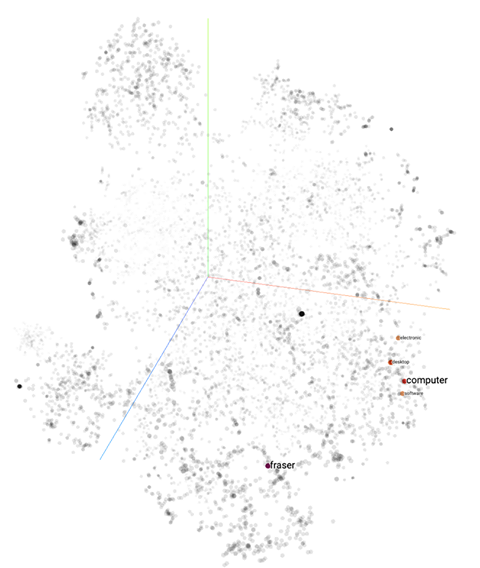
\includegraphics[width=\linewidth]{figures/computer_emb_neighbors.png}
%   \caption{A subfigure}
  \label{figure:car:neighborhood}
\end{subfigure}%
\begin{subfigure}{.5\textwidth}
  \centering
  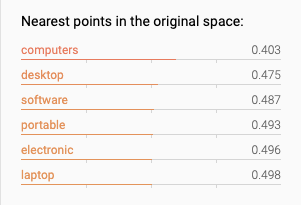
\includegraphics[width=\linewidth]{figures/computer_nearest_neighbors.png}
%   \caption{A subfigure}
  \label{figure:car:neighbor}
\end{subfigure}
\caption{Neighborhood of \emph{car} in the embedding space of AWD-LSTM.}
\label{figure:car}
\end{figure}

\begin{figure}
\centering
\begin{subfigure}{.5\textwidth}
  \centering
  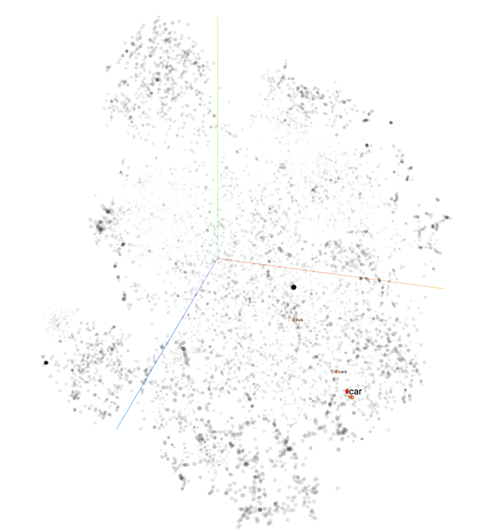
\includegraphics[width=\linewidth]{figures/car_emb_neighbor.png}
%   \caption{A subfigure}
  \label{figure:computer:neighborhood}
\end{subfigure}%
\begin{subfigure}{.5\textwidth}
  \centering
  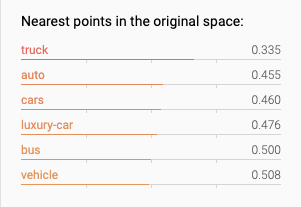
\includegraphics[width=\linewidth]{figures/car_nearest_neighbors.png}
%   \caption{A subfigure}
  \label{figure:computer:neighbor}
\end{subfigure}
\caption{Neighborhood of \emph{computer} in the embedding space of AWD-LSTM.}
\label{figure:computer}
\end{figure}

Now imagine every single word that can finish the previous sentence. Every one of those words is embedded into its own neighborhood where it is close to other words that share the same context on average. Therefore, a simple single mode Gaussian seems very limited for all those \emph{``fat tail''} situations in natural languages. Ideally, we would like something that can adapt based on the context, i.e. given a hidden state we can obtain different type of distributions. It is also possible that the success of MoS \citep{yang2017breaking} and DOC \citep{takase2018direct} papers, in addition to breaking the \emph{softmax bottleneck}, is due to the fact that they learn a dynamic mixture of Gaussians, which by definition is more expressive. Additionally, based on the amount of Gaussians in the mixture, those approaches are more or less capable of solving the previously mentioned issues.

To generalize, it seems unlikely that a single general distribution, conditioned on the hidden state, can capture all possible situations in Language Modelling. Therefore, it seems reasonable that based on the context, or the hidden state if you want, we would like to obtain custom distributions that specifically fit the need of the current context. But what if we can start with a ``simple'', single, general distribution and then based on the context, distort it into a more complex distribution if needed? That would alleviate the need to manually tune the amount of components in the mixture and can be seen as a generalization of MoS \citep{yang2017breaking} and DOC \citep{takase2018direct}.

\chapter{Related Work}
\label{chapter:related_work}

\section{AWD-LSTM}
\label{section:related_work:awd_lstm}
\citet{merity2017regularizing} had several crucial contributions to RNN-based language modelling with their AWD-LSTM model.

First, regularizing RNNs is a complicated matter. A na\"ive application of dropout \citep{srivastava2014dropout}, where we randomly dropout units in every time step, results in unit starvation and disrupts the RNN's ability to retain long term dependencies. \citet{gal2016theoretically} suggest using the same dropout mask in every time step, to prevent this from happening. On the other hand, \citet{merity2017regularizing} propose the weight-dropped LSTM, which uses Dropconnect \citep{wan2013regularization} on the hidden-to-hidden weights as a recurrent regularization.

Secondly, they propose the use of Non-monotonically Triggered Averaged Stochastic Gradient Descent (NT-ASGD) as an optimization algorithm, instead of the regular Stochastic Gradient Descent (SGD).

The training of neural networks can be defined as

\begin{displaymath}
    \hat{\theta} = \underset{\theta}{argmin} \ \frac{1}{N} \sum^N_{i=1} f_i(\theta),
\end{displaymath}

where $ f_i $ is the loss function for the $ i $-th data point and $ \theta $ are the parameters to be learned. SGD takes the form of

\begin{displaymath}
    \theta_{k+1} = \theta_k + \gamma_k \hat{\nabla} f(\theta_k),
\end{displaymath}

where $ k $ stands for the iteration number, $ \gamma_k $ is the learning rate and $ \hat{\nabla} $ denotes a stochastic gradient on a minibatch of samples. After convergence, SGD returns the final iteration as the solution. Contrary to this, Averaged SGD (ASGD) returns the average

\begin{displaymath}
    \frac{1}{K-T+1} \sum_{i=T}^K \theta_i
\end{displaymath}

as a solution. Here $ K $ is the total number of iterations and $ T < K $ is a user-specified averaging trigger. \citet{merity2017regularizing} propose to use an automatic trigger mechanism for the averaging. Instead of manually specifying a value for $ T $, they propose a non-monotonic criterion that triggers the averaging when the validation metric does not improve for several epochs. The full method is shown in algorithm \ref{algorithm:related_work:ASGD}.

\begin{algorithm}[H]
\SetAlgoLined
\SetKwInOut{Input}{Inputs}
\Input{Initial parameters $ \theta_0 $, learning rate $ \gamma $, logging interval $ L $, non-monotone interval $ n $}
 Initialize $k \leftarrow 0, \ t \leftarrow 0, \ T \leftarrow 0, \ logs \leftarrow [] $ \\
 \While{stopping criterion not met}{
  Compute stochastic gradient $ \hat{\nabla}f(\theta_k) $ and take the SGD step \\
  \If{mod(k, L) = 0 and T = 0}{
   Compute validation perplexity $ v $ \\
   \If{t $ > $ n and v $ > $ \ $ \underset{l \ \in \ {t-n, \ ... , \ t}}{min} \ logs[l] $ }{
    Set $ T \leftarrow K $
   }
   Append $ v $ to $ logs $ \\
   $ t \leftarrow t + 1 $
   }
 }
 \Return $ \frac{1}{k - T + 1} \sum_{i=T}^k \theta_i $
 \caption{Non-monotonically Triggered ASGD (NT-ASGD) \citep{merity2017regularizing}\label{algorithm:related_work:ASGD}}
\end{algorithm}

Finally, their codebase \footnote{https://github.com/salesforce/awd-lstm-lm} set a new foundation for RNN-based language modelling. Every other notable model that came out in the next few years used their codebase as a basis to build upon.

\section{Mixture of Softmaxes}
\label{section:related_work:mos}

\citet{yang2017breaking} contributions in their paper \emph{Breaking the Softmax Bottleneck} are two-fold. First, they identify the Softmax Bottleneck problem described in section \ref{section:limitations:softmax_bottleneck} and secondly, they propose a simple technique that allows to bypass this limitation.

They use the AWD-LSTM model to encode the context in a vector $ g_c $. Then, they project $ g_c $ to obtain multiple hidden states

\begin{displaymath}
    h_{c, k} = tanh(W_{h,k} g_c)
\end{displaymath}

where $ h_{c, k} $ stands for the $ k $-th component for context $ c $ and $ W_k $ are trainable parameters. Then, the conditional probability of a word given a context is modelled as

\begin{align*}
    P_\theta(w | c) = &\sum_{k=1}^K \pi_{c, k} \frac{\exp{h^T_{c, k} e_w}}{\sum_{w'} \exp{h^T_{c, k} e_{w'}}} \\
    s.t. &\sum_{k=1}^K \pi_{c, k} = 1,
\end{align*}

where $ e_w $ is the (output) word embedding for word $ w $. The prior weights $ \pi_{c, k} $ are obtained by

\begin{displaymath}
    \pi_{c, k} = \frac{\exp{w_{\pi, k}^T g_c}}{\sum_{k'=1}^K \exp{w_{\pi, k'}^T g_c}}.
\end{displaymath}

According the previous equations, we can deduce that \citet{yang2017breaking} propose to have a weighted average between several Softmax functions. Therefore, they call this model \emph{Mixture of Softmaxes (MoS}. Furthermore, if we create a matrix $ \hat{A}_{MoS} $ similar to the one in section \ref{section:limitations:softmax_bottleneck}, we get

\begin{displaymath}
    \hat{A}_{MoS} = \log \sum_{k=1}^K \Pi_k \exp (H_{k}E).
\end{displaymath}

As $ \hat{A}_{MoS} $ is now obtained via a non-linear transformation, we can deduce that its rank is not bounded and $ \hat{A}_{MoS} $ can potentially be a full-rank matrix.

\section{Direct Output Connections}
\label{section:related_work:doc}

\citet{takase2018direct} propose their \emph{Direct Output Connections (DOC)} model as a generalization of MoS. DOC computes $ J $ probability distributions from all layers and performs a weighted average between them. The output probabilities in DOC, are computed as

\begin{align*}
    P_\theta(w | c) = &\sum_{j=1}^J \pi_{j, c} \ Softmax(\Tilde{W}k_{j,c}) \\
    s.t. &\sum_{j=1}^J \pi_{j, c} = 1
\end{align*}

where $ \pi_{j, c} $ is the weight for the $ j $-th component in the mixture given context $ c $ and is obtained by

\begin{displaymath}
    \pi_{c} = Softmax(W_\pi h^N_c),
\end{displaymath}

where $ \pi_{c} $ is a vector with elements $ \pi_{j, c} $, $ W_\pi $ is a weight matrix and $ h^N $ is the hidden state from the final layer. Furthermore, $ \Tilde{W} \in R^{|V| \times d} $ is a weight matrix and $ k_{j,c} \in R^d $ is a vector computed from the hidden state of some layer $ n $ as

\begin{displaymath}
    k_{j, c} = W_j h^n_c.
\end{displaymath}

In this equation $ W_j \in R^{d \times d_{h^n}} $ is a weight matrix. Additionally, let $ i_n $ be the number of $ k $-s computed from the hidden state of the $ n $-th layer s.t. $ \sum_{n=0}^N i_n = J $. From here we can deduce that for $ i_N = J $, i.e. if all distributions are obtained from the final layer, DOC is equivalent to MoS, which is exactly why DOC is considered to be a generalization of MoS.

Finally, if we construct the matrix containing all log-probabilities given all contexts for DOC, we can notice that it takes the form of

\begin{displaymath}
    \hat{A} = \log \sum_{j=1}^J \Pi \ Softmax(K_j \Tilde{W}^T)
\end{displaymath}

where $ \Pi $ is a diagonal matrix whose entries are the weights $ \pi_{j, c} $ and $ K_j $ is a matrix whose rows are vectors $ k_{j,c} $. As $ \hat{A} $ is obtained using a non-linear transformation, $ \hat{A} $ can be of an arbitrary high rank is not limited by the Softmax Bottleneck explained in section \ref{section:limitations:softmax_bottleneck}.

\chapter{Neural Ordinary Differential Equations}
\label{chapter:ode}

\section{Introduction to Neural ODEs}
\label{section:ode:introduction}

In recent years Residual Networks (ResNet) \citep{he2016deep} have brought a great success in Deep Learning and especially in computer vision. They have proven to be effective against the vanishing gradient and the degradation problems and have drastically eased the optimization of very deep neural networks. If we refer to the output vector of each layer as $ z_t $ where $ t $ stands for the layer, then Residual Networks can be mathematically described as

\begin{equation}
    \label{equation:ode:resnet}
    z_{t+1} = z_{t} + f(z_{t}; \ \theta_{t}),
\end{equation}

where $ t \in \{0, ..., T\} $, $ z_t \in R^D $ and $ \theta_t $ are the parameters of the \emph{t}-th layer. These iterative updates can be interpreted as an Euler discretization of a continuous transformation \citep{lu2017beyond, haber2017stable, ruthotto2018deep}.

Moreover, as we add more layers and take smaller steps, in the limit, we parameterize the continuous dynamics of the hidden state using an ordinary differential equation (ODE) specified by a neural network

\begin{equation}
    \label{equation:ode:odes}
    \frac{d z(t)}{d t} = f(z(t), \ t; \ \theta ).
\end{equation}

\citet{chen2018neural} introduced this concept as a new family of deep neural network models, where the neural network outputs the gradient of the hidden state with respect to the depth. Then, given an initial state and the differential equation parameterized by the neural network, the final state is obtained by solving an ODE. The analogy they make is the one that considers this family of models to be the continuous case of ResNets. Figure \ref{figure:ode:resnet_vs_ode}, depicts the similarities and differences between ResNets and neural networks based on ODEs. They call this family of models \emph{Neural ODEs} or \emph{ODENets}, and provide an open source framework implemented in PyTorch\footnote{\url{https://github.com/rtqichen/torchdiffeq}}.

\begin{figure}[ht]
      \centering
      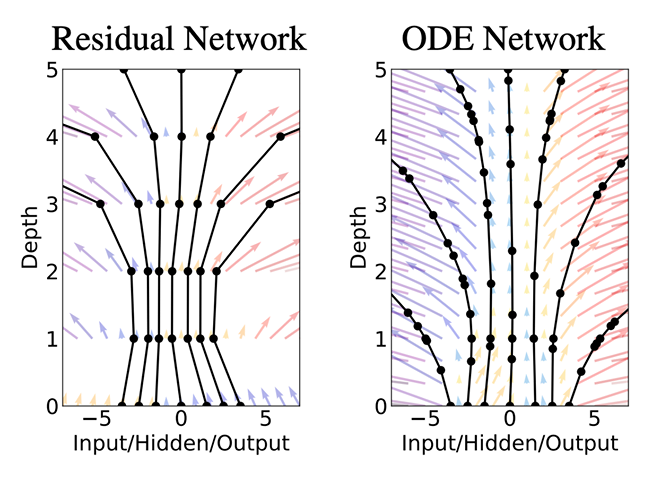
\includegraphics[width=0.7\columnwidth]{figures/resnet_vs_odes.png}
      \caption{\emph{Left}: A Residual network defines a discrete sequence of finite transformations. \emph{Right}: An ODE network defines a vector field that continuously transforms the state \citep{chen2018neural}.}
      \label{figure:ode:resnet_vs_ode}
\end{figure}

In equation \ref{equation:ode:odes}, $ z(t) $ is the hidden state in the \emph{t}-th layer, and $ f $ can be any neural network parameterized by $ \theta $, with $ z(t) $ and $ t $ as inputs and the gradient of $ z(t) $ with respect to $ t $ as output. Furthermore, the final output of such a model can then be defined as

\begin{align}
    z(t_1) & = z(t_0) + \int_{t_0}^{t_1} \frac{d z(t)}{d t} \ dt \\
    & = z(t_0) + \int_{t_0}^{t_1} f(z(t), \ t; \ \theta ) \ dt \\
    & = ODESolve(z(t_0), f, t_0, t_1).
\end{align}

According to the equations above, we can conclude that, $ f $ is learning a vector field, which is why Neural ODEs can potentially be seen as models with infinite amount of layers. To be specific, the number of layers is dynamically decided and delegated to the ODE solver. Furthermore, \citet{chen2018neural} developed their framework in way that any ODE solver can be used as a blackbox. This allows for more flexibility and decouples the framework from the ODE solver. General purpose ODENets are illustrated on Figure \ref{figure:ode:odenets_visualization}.

\begin{figure}[ht]
      \centering
      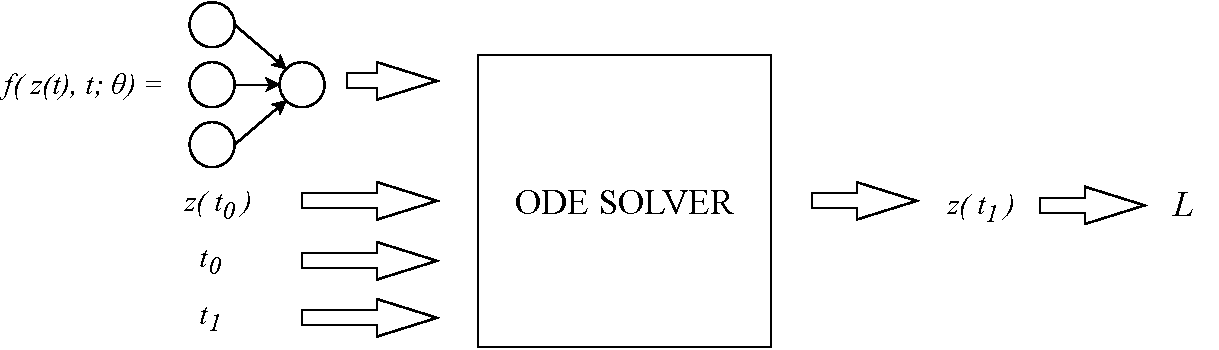
\includegraphics[width=\columnwidth]{figures/odenets_visualization.pdf}
      \caption{General purpose ODENet. $f(z(t), \ t; \ \theta) $ is neural network specifying the differential equation, $ z(t_0) $ is the initial state, $ t_0 $ is the initial time, $ t_1 $ is the final time, $ z(t_1) $ is the final state and $ L $ is a scalar valued loss function.}
      \label{figure:ode:odenets_visualization}
\end{figure}

Defining neural network models in this fashion has several advantages \cite{chen2018neural}:
\begin{itemize}
    \item \textbf{Memory Efficiency.} In section \ref{section:ode:backpropagation} it is discussed how circumventing backpropagation through the operations of the ODE solver saves a lot of memory.
    \item \textbf{Adaptive Computation.} Nowadays, ODE solvers provide guarantees about the growth of the approximation error, monitor the error, and adapt their evaluation strategy on the fly to achieve the required level of accuracy. This allows for explicit control over the speed versus precision trade-off.
    \item \textbf{Parameter Efficiency.} In section 3 of their work, \citet{chen2018neural} demonstrate how this family of models ties the weights of nearby layers, resulting in fewer parameters without the loss of performance.
    \item \textbf{Scalable and invertible normalizing flows.} Chapter \ref{chapter:cnf} sshows how one side effect of going in the continuous domain, allows for an easier and unrestricted use of normalizing flows. As a result, normalizing flows can be used for language modelling, as shown in chapter \ref{chapter:cnf_lm}.
    \item \textbf{Continuous time-series models.} RNNs are the de-facto architecture for time-series models. Unfortunately, they require that the observations are discretized and bound to specific emission intervals. On the other hand, continuously defined dynamics can naturally take care of observations that arrive at arbitrary times.
\end{itemize}

\section{Backpropagation through the ODE solver}
\label{section:ode:backpropagation}

An immediate question that rises, is how does one backpropagate through the ODE solver. In theory one can simply backpropagate through the operations of the solver, however, this has several drawbacks. First, some solvers, require solving a nonlinear optimization problem at every step. This can make direct backpropagation through the integrator difficult. Additionally, as mentioned in the previous section, ODENets can potentially have a very high number of layers. Backpropagating through such a large number of layers is inefficient from a memory point of view, as it would mean that all intermediate steps should be kept in memory until the backward pass is over. Therefore, what \citet{chen2018neural} propose, is to compute gradients by solving a second augmented ODE backwards in time. This method is called the \emph{adjoint sensitivity method} \citep{pontryagin2018mathematical} and is applicable to all ODE solvers. It scales linearly with problem size, has low memory cost, and allows for explicit control over numerical errors.

\begin{figure}[ht]
      \centering
      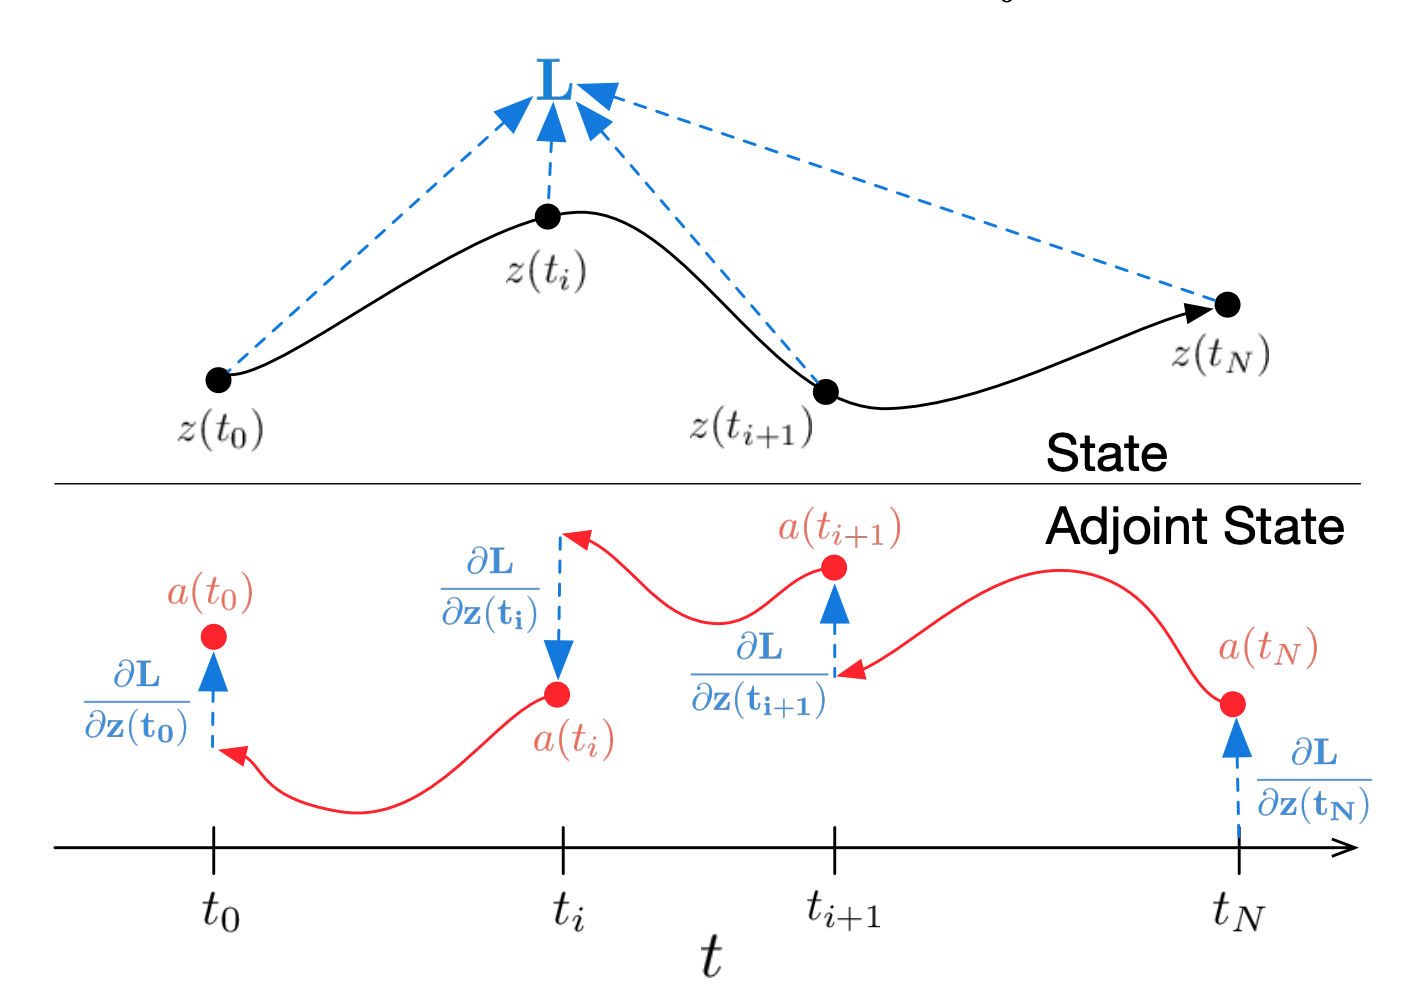
\includegraphics[width=\columnwidth]{figures/adjoint_method.png}
      \caption{Reverse-mode differentiation of an ODE solution. The adjoint sensitivity method solves an augmented ODE backwards in time. The red lines denote the sequence of separate ODE solves \cite{chen2018neural}.}
      \label{ode:adjoint}
\end{figure}

As shown in figure \ref{figure:ode:odenets_visualization}, we need to optimize a scalar valued loss function $ L $ whose input is the output of the ODE Solver.

\begin{equation}
    L(z(t_1)) = L \left( z(t_0) + \int_{t_0}^{t_1} f(z(t), \ t; \ \theta ) \right) = L(ODESolve(z(t_0), f, t_0, t_1))
\end{equation}

The parameters of the ODENet are the parameters of the neural network $ f $, which is why we are interested in the derivative of the loss function with respect to $ \theta $. \citet{pontryagin2018mathematical} show that the derivative takes the form of another initial value problem

\begin{equation}
    \label{loss_derivative}
    \frac{dL}{d\theta} = - \int_{t_1}^{t_0} \left(\frac{\partial L}{\partial z(t)}\right)^T \frac{\partial f(z(t), \ t; \ \theta)}{\partial \theta}dt
\end{equation}

Where $ \nicefrac{\partial L}{\partial z(t)} $ is known as the \emph{adjoint state} of the ODE. \citet{chen2018neural} use one call to an ODE solver to get $ z(t_1) $ and then a second one to calculate the equation \ref{loss_derivative}. In cases where the loss depends not only on the final state $ z(t_1) $, but also on the intermediate states $ z(t) $, the reverse-mode derivative must be broken into a sequence of separate solves as shown on figure \ref{ode:adjoint}.

\section{Neural ODEs for Language Modelling}
\label{section:ode:ode_lms}

We can look at language modelling as a two step process. First, we encode the context into a hidden state vector, and then using the hidden state vector we generate a distribution over the vocabulary. The former is commonly done by an LSTM-based RNN. Then, given the hidden state, a Softmax layer is used to obtain the probability distribution over the vocabulary. In section \ref{section:limitations:softmax_bottleneck}, it is discussed how having this Softmax layer introduces a theoretical limitation on LMs, and in sections \ref{section:related_work:mos} and \ref{section:related_work:doc} is discussed how models like MoS \citep{yang2017breaking} and DOC \citep{takase2018direct} have tried to break it. In this section, a simple model based on Neural ODEs is proposed, that is not restricted by the Softmax Bottleneck problem.

Let $ V $ be the vocabulary, $ h $ be the hidden state, $ d $ be the hidden state dimensionality, $ L \in R^{d \times |V|} $ be the output projection matrix (if weights are tied \citep{inan2016tying} this is also the embedding matrix), and $ y^* \in R^{|V|} $ be a one-hot encoded ground truth vector. The model can then be represented as

\begin{align*}
    l(t_0) &= L^T h, \ l \in R^{|V|} \\
    l(t_1) &= node(l(t_0), \ f) \\
    y &= Softmax(l(t_1)),
\end{align*}

where $ node $ is a NeuralODE block defined as

\begin{displaymath}
    node(l(t_0), \ f) = l(t_0) + \int_{t_0}^{t_1} f(l(t), \ t) dt    
\end{displaymath}

and $ f $ is a neural network parameterizing the gradient of the logits $ l $ with respect to time or in this case depth. Moreover, $ f $ can be an arbitrary neural network architecture and one possibility is to define it as

\begin{displaymath}
    f(l, t) = H_f ReLU(W_f^T l), \ W_f, H_f \in R^{|V| \times |V|}.    
\end{displaymath}

An apparent problem with this approach lies in the $ W_f, H_f \in R^{ |V| \times |V| } $ matrices. As the vocabulary can often be in the tens of thousands, this highly increases both the memory and the time complexity of the overall model. However, this problem can be solved by using a dimensionality bottleneck:

\begin{displaymath}
    f(l, t) = H_f ReLU(W_f^T l), \ W_f, H_f \in R^{|V| \times k},
\end{displaymath}

where $ k $ is the dimensionality of the bottleneck and is usually in the low hundreds.

In the simplest form of $ f $, $ t $ can be ignored. This is the same as stating that the gradient does not depend on it and we have a constant vector field as we move through time. Other possibilities are to concatenate it to the input or use it in a conjunction with Hypernetworks \citep{ha2016hypernetworks} to generate $ W_f $ and $ H_f $ based on $ t $. Both approaches are suggested in \citet{chen2018neural} and \citet{grathwohl2018ffjord}. Finally, we can use \emph{Cross-Entropy} for training.

The main idea behind this approach is to solve the Softmax Bottleneck by applying non-linear transformations on the logits, similarly to what is done in \citep{ganea2019breaking}. The difference between the two approaches lies in the nature of the non-linearities applied. \citet{ganea2019breaking} apply monotonic pointwise non-linearities, and here we use a Neural ODE.

\chapter{Neural Ordinary Differential Equations for Language Modelling}
\chapter{Continuous Normalizing Flows}
\label{chapter:cnf}

\section{Introduction to Normalizing Flows}
\label{section:cnf:normalizing_flows}

Section ends with a question: "What if we can start with a simple distribution and distort it into a more complex one?". To answer this question, let us first examine what happens with the densities as we transform some random variable.

Let $ x \in R^d $ be a random variable with an underlying probability density function $ P_x $ and $ f: R^d \mapsto R^d $ be an invertible transformation. Then, if

\begin{displaymath}
    y = f(x),
\end{displaymath}

i.e. we obtain the random variable $ y $ by transforming $ x $ using $ f $, the probability density function $ P_y $ of $ y $ can be obtained using the change of variables formula

\begin{equation}
    \label{equation:cnf:nf:change_density}
    P_y(y) = P_x(x) \left | det \frac{\partial f}{\partial x} \right |^{-1}
\end{equation}

and the change in log density becomes

\begin{equation}
    \label{equation:cnf:nf:change_log_density}
    \log P_y(y) = \log P_x(x) - \log \left | det \frac{\partial f}{\partial x} \right |.
\end{equation}

Now let us assume that instead of a single transformation, we want to apply a series of transformations. Let $ f_i: R^d \mapsto R^d, \ i \in \{1, \ ..., \ n\} $ be $ n $ different transformations, and let $ z_0 $ be an initial random variable with a probability density function $ P_{z_0} $. Then, we can denote the composition of functions $ f_i $ on $ z_0 $ as

\begin{displaymath}
    z_n = f_n \circ ... \circ f_1(z_0),
\end{displaymath}

with the probability density function of $ z_n $ being

\begin{equation}
    \label{equation:cnf:nf:total_change_density}
    P_{z_n}(z_n) = P_{z_0}(z_0) \prod_{i=1}^n \left | det \frac{\partial f_i}{\partial z_{i-1}} \right |^{-1}
\end{equation}

and the total change in log density being

\begin{equation}
    \label{equation:cnf:nf:total_change_log_density}
    \log P_{z_n}(z_n) = \log P_{z_0}(z_0) - \sum_{i=1}^n \log \left | det \frac{\partial f_i}{\partial z_{i-1}} \right |.
\end{equation}

This technique is called a normalizing flow and was formalized by \citet{rezende2015variational}. They start with a simple probability density function and transform it into a more complex one, by applying a sequence of invertible transformations until a desired level of complexity is obtained. Some simple normalizing flows introduced in their paper \citep{rezende2015variational} are the \emph{planar} and the \emph{radial} flow. The transformation for the planar flow is

\begin{displaymath}
    f(z) = z + uh(w^Tz + b),
\end{displaymath}

where $ u, w \in R^d, b \in R $ and $ h $ is a smooth element-wise non-linearity. On the other hand, the transformation of the radial flow is

\begin{displaymath}
    f(z) = z + \beta h(\alpha, r)(z - z_0),
\end{displaymath}

where $ z_0 \in R^d, \ \alpha \in R^+, \ \beta \in R, \ r = \lvert z - z_0 \rvert $ and $ h(\alpha, \ r) = \nicefrac{1}{\alpha + r} $. The planar flow introduces hyperplanes into the space, and the radial flow introduces spheres into the space.

\begin{figure}[ht]
      \centering
      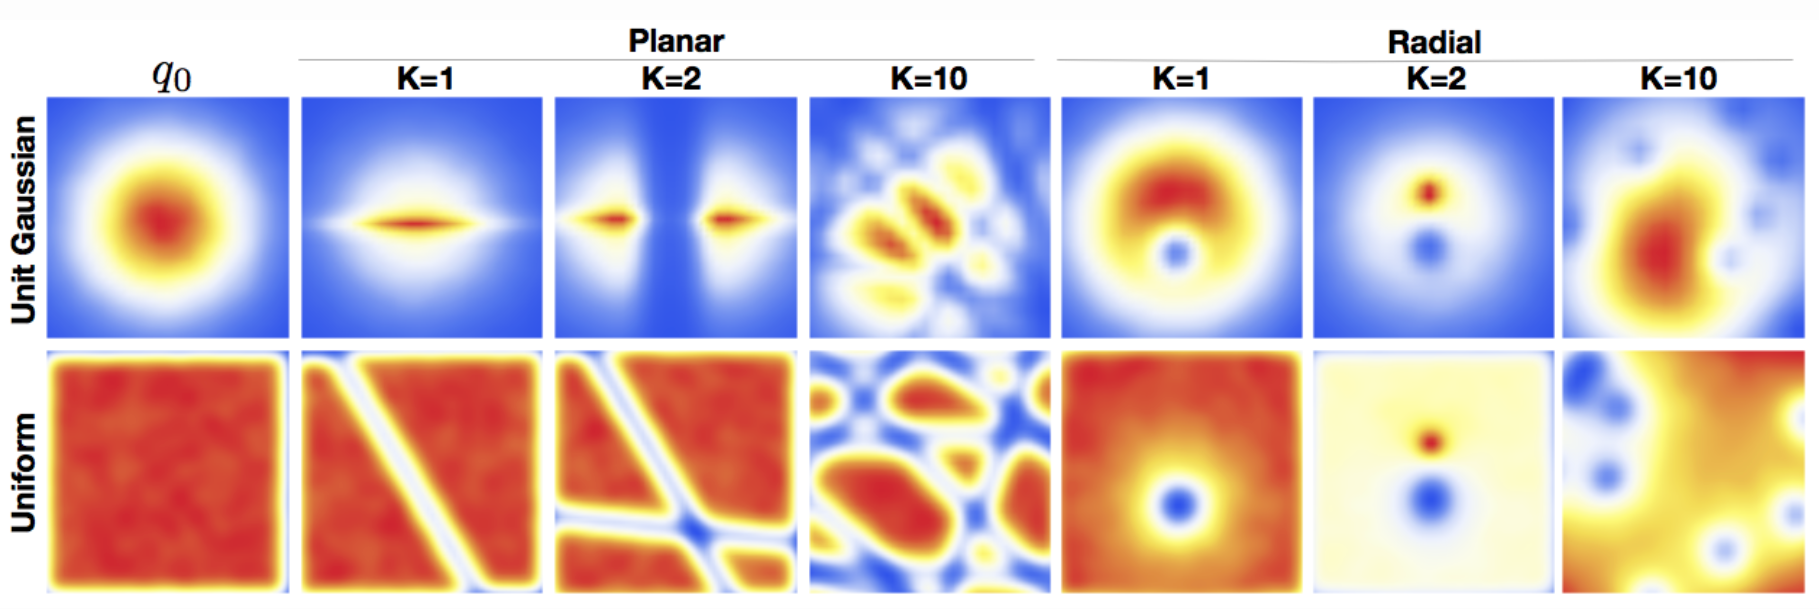
\includegraphics[width=\columnwidth]{figures/planar_radial_flows.png}
      \caption{The effect of planar and radial flows on uniform and unit Gaussian distributions \citep{rezende2015variational}.}
      \label{figure:cnf:planar_radial_flows}
\end{figure}

However, in practice, normalizing flows are limited due to their high computational complexity. By looking at equations \ref{equation:cnf:nf:change_density} up to \ref{equation:cnf:nf:total_change_log_density}, we can deduce that normalizing flows require calculating a determinant, which is generally a $ \mathcal{O}(d^3) $ operation. Therefore, their expressiveness is limited by the need to use relatively simple transformations, which Jacobians are easy to compute. For example, both the planar and radial flow allow for linear cost determinant computation and their effect are illustrated on figure \ref{figure:cnf:planar_radial_flows}.

\section{Continuous Normalizing Flows}
\label{section:cnf:cnf}

The previous chapter introduces a novel family of neural models under the name NeuralODEs. \citet{chen2018neural} noticed that the discretized equation \ref{equation:ode:resnet} also appears in Normalizing Flows \citep{rezende2015variational} and the NICE framework \citep{dinh2014nice}. They further realized that performing continuous transformations has an unexpected side effect to the change of variables formula.

\begin{figure}[ht]
      \centering
      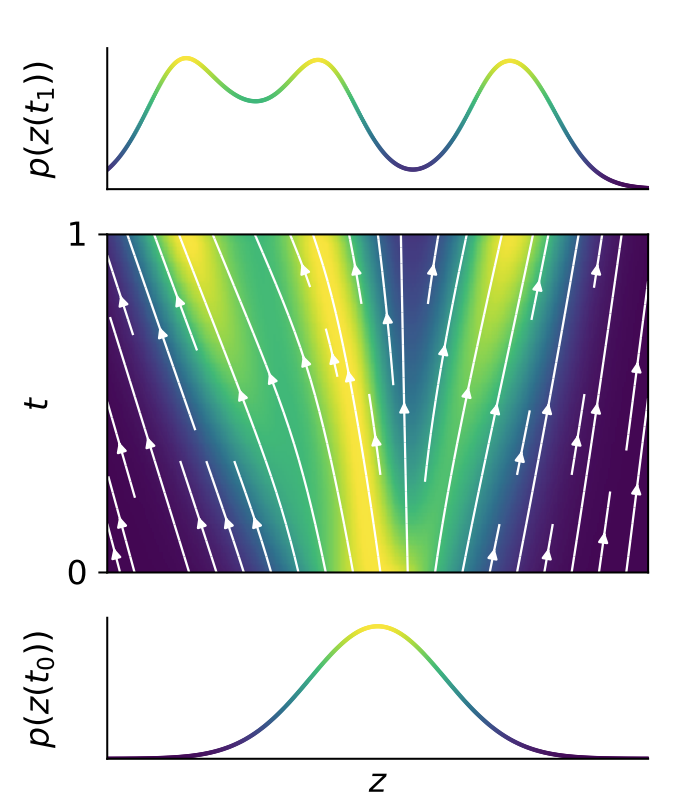
\includegraphics[width=0.5\columnwidth]{figures/cnf_transformations.png}
      \caption{Continuous Normalizing Flows distorting a single mode Gaussian into a more complex distribution \citep{grathwohl2018ffjord}}
      \label{figure:cnf:cnf_transformations}
\end{figure}

Recall from equation \ref{equation:cnf:nf:change_log_density}, that when applying discrete transformations, the change in log density is given by

\begin{align}
    z_{1} &= f(z_{0}), \\
    \log p(z_{1}) &= \log p(z_{0}) - \log \left \lvert det \frac{\partial f}{\partial z_{0}} \right \rvert,
\end{align}

however, when going into the continuous domain, the change in log density becomes

\begin{align}
    \frac{\partial z(t)}{\partial t} &= f(z(t), t), \\
    \frac {\partial \log p(z(t))} {\partial t} &= -Tr \left( \frac{\partial f}{\partial z(t)} \right),
\end{align}

with the total change in log density given by

\begin{displaymath}
    \log p(z(t_1)) = \log p(z(t_0)) - \int_{t_0}^{t_1} Tr \left( \frac{\partial f}{\partial z(t)} \right) dt    
\end{displaymath}

This combination of NeuralODEs and Normalizing Flows is called \emph{Continuous Normalizing Flows (CNFs)} and can be visualized on Figure \ref{figure:cnf:cnfs_visualization}. One huge difference in the continuous case, is that instead of computing the determinant of the Jacobian, we only need to calculate the trace. Determinants are generally calculated in $ \mathcal{O}(d^3) $, however, the trace is a linear cost operation.

\begin{figure}[ht]
      \centering
      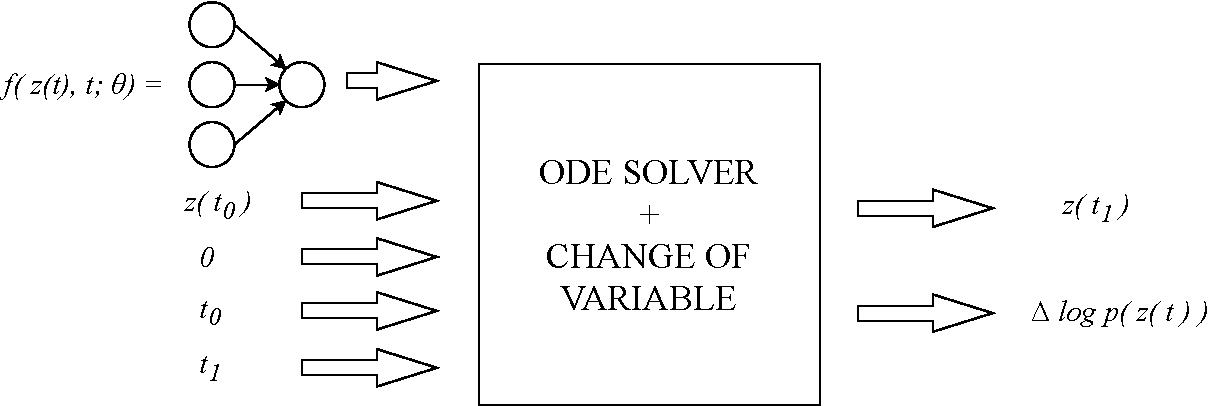
\includegraphics[width=\columnwidth]{figures/cnfs_visualization.pdf}
      \caption{$f(z(t), \ t; \ \theta) $ is neural network specifying the differential equation, $ z(t_0) $ is the initial state, $ 0 $ is the initial log-density, $ t_0 $ is the initial time, $ t_1 $ is the final time, $ z(t_1) $ is the final state and $ \Delta \log p(z(t)) $ is the change in log-density.}
      \label{figure:cnf:cnfs_visualization}
\end{figure}

Unfortunately, the overall complexity of the method above is still $ \mathcal{O}(d^2) $ due to the Jacobian, which even though better, is still restrictive. \citet{grathwohl2018ffjord} further optimize the above method and reduce the overall complexity to $ \mathcal{O}(d) $. They achieve this in two steps. First, Vector-Jacobian products can be computed efficiently using reverse-mode automatic differentiation. Secondly, they show that they can get unbiased estimates of the trace of the Jacobian, by using the Hutchinson’s trace estimator \citep{hutchinson1990stochastic}. Consequently, they claim that Continuous Normalizing Flows implemented in this fashion can be considered unrestricted due to the free-form Jacobian of the transformation $ f $.

\citet{grathwohl2018ffjord} additionally provide a PyTorch framework \footnote{https://github.com/rtqichen/ffjord/} with the previously mentioned improvements. Within their framework we can apply CNFs to random variables and log densities as

\begin{displaymath}
    \underbrace{
        \begin{matrix}
            \begin{bmatrix}
                z(t_1) \\
                \Delta \log p(z_t) %\log p(z_{t_1}) - \log p(z_{t_0})
            \end{bmatrix}
        \end{matrix}
    }_{Solution}
    =
        \bigintss_{t_0}^{t_1}
        \underbrace{
            \begin{matrix}
                \begin{bmatrix}
                    f(z(t), t; \theta) \\
                    Tr \left ( \frac{\partial f}{\partial z(t)} \right)
                \end{bmatrix}
            \end{matrix}
    }_{Dynamics}
    dt = cnf
    \Bigg (
        \underbrace{
            \begin{matrix}
                \begin{bmatrix}
                    z(t_0) \\
                    0
                \end{bmatrix}
            \end{matrix},
        }_{Initial Values}
        t_0, \ t_1, \ f
    \Bigg )
\end{displaymath}

and finally we can obtain $ \log p(z_{t_1}) $  as 

\begin{displaymath}
    \log p(z_{t_1}) = \log p(z_{t_0}) - \Delta \log p(z_t).
\end{displaymath}

\chapter{Continuous Normalizing Flows for Language Modelling}
\chapter{Models}
\chapter{Experiments}

%%%%%%%%%%%%%%%%%%%%%%%%%%%%%%%%%%%%%%%%%%%%%%%%%%%%%%%%%%%%%%%%%%%%%%%%%%
\section{Legend}
This section explains the abbreviations in the tables below mean.

\begin{itemize}
    \item \emph{model} - the model being used. AWD stands for AWD-LSTM \citep{merity2017regularizing}, MoS \citep{yang2017breaking} stands for Mixture of Softmaxes and DoC stands for Direct Output Connections \citep{takase2018direct}.
    \item \emph{exp} - number of experts. Models that perform a mixture of distributions need a prespecified value for the number of components in the mixture.
    \item \emph{h} - dimensionality of the middle hidden states of the RNN.
    \item \emph{lasth} - dimensionality of the final hidden state of the RNN.
    \item \emph{emb} - dimensionality of the embeddings.
    \item \emph{lr} - learning rate.
    \item \emph{ep} - epoch at which the presented results are obtained.
    \item \emph{vloss / tloss} - validation loss / test loss. Loss obtained on the validation or the test set.
    \item \emph{vppl / tppl} - validation perplexity / test perplexity. Perplexity obtained on the validation or the test set.
    \item \emph{vbpc / tbpc} - validation bits per character / test bits per character. Bits per character obtained on the validation or the test set.
    \item \emph{prefinetuned} - in the case of transfer learning specifies whether the base model was finetuned before transferring the weights.
    \item \emph{freeze} - in the case of transfer learning specifies whether the transfered weights are fixed or trainable.
\end{itemize}

\section{Datasets}
All models are evaluated on the Penn Treebank dataset which is the standard dataset for evaluating language models. The dataset is used as preprocessed by \citet{mikolov2011empirical} and it consists of 929k training words, 73k validation words, and 82k test words. After preprocessing, all words consist of only lowercase letters and all numbers are replaced with a placeholder $ N $. Additionally, newlines are replaced with a special \textless eos\textgreater \ token. Finally, after preprocessing the dataset contains only the 10k most frequent words and the rest are replaced with a special \textless unk\textgreater \ token.

%%%%%%%%%%%%%%%%%%%%%%%%%%%%%%%%%%%%%%%%%%%%%%%%%%%%%%%%%%%%%%%%%%%%%%%%%%
\section{Word Based Models}

\subsection{Baselines}

The following three models were used as baselines

\begin{enumerate}
    \item AWD-LSTM \citep{merity2017regularizing}
    \item MoS \citep{yang2017breaking}
    \item DOC \citep{takase2018direct}
\end{enumerate}

For every baseline the latest hyperparameters proposed in their corresponding github repositories were used. Unfortunately, due to changes in PyTorch versions, exact reproduction of their results was not possible. The results before finetuning can be seen in table \ref{table:experiments:baselines_word} and the results after finetuning can be seen in table \ref{table:experiments:baselines_word_finetuned}.

\begin{table}[]
% \centering
\caption{Results from baseline word-based models before finetuning.}
\begin{tabular}{|l|l|l|l|l|l|l|l|l|l|l|}
\hline
\textbf{model}    & \textbf{exp} & \textbf{h}   & \textbf{lasth} & \textbf{emb} & \textbf{lr} & \textbf{ep}  & \textbf{vloss} & \textbf{vppl}  & \textbf{tloss} & \textbf{tppl}  \\ \hline
AWD      & n/a & 960 & 400   & 400 & 20 & 517 & 4.11  & 60.93 & 4.07  & 58.67 \\ \hline
MoS      & 15  & 960 & 620   & 280 & 20 & 511 & 4.06  & 57.89 & 4.02  & 55.84 \\ \hline
DoC      & 15  & 960 & 620   & 280 & 20 & 500 & 4.02  & 55.45 & 3.98  & 53.44 \\ \hline
\end{tabular}
\label{table:experiments:baselines_word}
\end{table}

\begin{table}[]
\centering
\caption{Results from baseline word-based models after finetuning.}
\begin{tabular}{|l|l|l|l|l|}
\hline
\textbf{model} & \textbf{vloss} & \textbf{vppl}  & \textbf{tloss} & \textbf{tppl}  \\ \hline
AWD   & 4.10  & 60.33 & 4.06  & 58.05 \\ \hline
MoS   & 4.04  & 56.73 & 4.00  & 54.54 \\ \hline
DoC   & 4.00  & 54.68 & 3.97  & 52.87 \\ \hline
\end{tabular}
\label{table:experiments:baselines_word_finetuned}
\end{table}

\subsection{NeuralODE Logit Transformations}

\begin{table}[]
\centering
\caption{Results from performing NeuralODE-based transformations on top of the logits of a pretrained AWD-LSTM model.}
\begin{tabular}{|l|l|l|l|l|l|l|l|}
\hline
\textbf{prefinetuned} & \textbf{freeze} & \textbf{lr} & \textbf{ep} & \textbf{vloss} & \textbf{vppl} & \textbf{tloss} & \textbf{tppl} \\ \hline
no        & no        & 0.01      & 12        & 4.09      & 59.94     & 4.06      & 57.71 \\ \hline
yes       & no        & 0.01      & 5         & 4.10      & 60.50     & 4.06      & 58.09 \\ \hline
no        & yes       & 0.01      & 4         & 4.11      & 60.73     & 4.07      & 58.68 \\ \hline
yes       & yes       & 0.01      & 4         & 4.10      & 60.56     & 4.06      & 58.25 \\ \hline
no        & no        & 0.1       & 1         & 4.09      & 60.02     & 4.06      & 57.73 \\ \hline
yes       & no        & 0.1       & 1         & 4.11      & 60.79     & 4.06      & 58.25 \\ \hline
no        & yes       & 0.1       & 1         & 4.11      & 60.80     & 4.07      & 58.74 \\ \hline
yes       & yes       & 0.1       & 1         & 4.11      & 60.65     & 4.07      & 58.33 \\ \hline
\end{tabular}
\end{table}


\subsection{Continuous Normalizing Flows}


\subsubsection{Basic CNFs}

\begin{table}[]
\centering
\caption{Results from training CNFs on top of a pretrained AWD-LSTM word-based model.}
\begin{tabular}{|l|l|l|l|l|l|l|l|}
\hline
\textbf{prefinetuned} & \textbf{freeze} & \textbf{lr} & \textbf{ep} & \textbf{vloss} & \textbf{vppl} & \textbf{tloss} & \textbf{tppl}  \\ \hline
no        & no        & 0.1       & 152       & 4.12      & 61.56     & 4.07      & 58.80 \\ \hline
yes       & no        & 0.1       & 160       & 4.15      & 63.20     & 4.11      & 60.97 \\ \hline
no        & yes       & 0.1       & 80        & 4.11      & 60.65     & 4.07      & 58.53 \\ \hline
yes       & yes       & 0.1       & 44        & 4.10      & 60.51     & 4.06      & 58.21 \\ \hline
no        & no        & 1         & 73        & 410       & 60.58     & 4.06      & 57.88 \\ \hline
yes       & no        & 1         & 43        & 4.11      & 60.98     & 4.07      & 58.28 \\ \hline
no        & yes       & 1         & 27        & 4.11      & 61.06     & 4.07      & 58.75 \\ \hline
yes       & yes       & 1         & 21        & 4.12      & 61.31     & 4.08      & 58.88 \\ \hline

\end{tabular}
\end{table}


\begin{table}[]
\centering
\caption{Results from training CNFs on top of a pretrained MoS word-based model.}
\begin{tabular}{|l|l|l|l|l|l|l|l|}
\hline
\textbf{prefinetuned} & \textbf{freeze} & \textbf{lr} & \textbf{ep} & \textbf{vloss} & \textbf{vppl} & \textbf{tloss} & \textbf{tppl} \\ \hline
no        & no        & 0.01      & 61        & 4.07      & 58.62     & 4.03      & 56.45 \\ \hline
yes       & no        & 0.01      & 58        & 4.06      & 57.80     & 4.02      & 55.46 \\ \hline
no        & yes       & 0.01      & 355       & 4.06      & 57.70     & 4.02      & 55.78 \\ \hline
yes       & yes       & 0.01      & 338       & 4.04      & 56.65     & 4.00      & 54.53 \\ \hline
no        & no        & 0.1       & 7         & 4.09      & 59.49     & 4.05      & 57.29 \\ \hline
yes       & no        & 0.1       & 7         & 4.07      & 58.77     & 4.03      & 56.35 \\ \hline
no        & yes       & 0.1       & 62        & 4.05      & 57.56     & 4.02      & 55.68 \\ \hline
yes       & yes       & 0.1       & 62        & 4.03      & 56.50     & 4.00      & 54.42 \\ \hline
\end{tabular}
\end{table}

\begin{table}[]
\centering
\caption{Results from training CNFs on top of a pretrained DoC word-based model.}
\begin{tabular}{|l|l|l|l|l|l|l|l|}
\hline
\textbf{prefinetuned} & \textbf{freeze} & \textbf{lr} & \textbf{ep} & \textbf{vloss} & \textbf{vppl} & \textbf{tloss} & \textbf{tppl} \\ \hline
no           & no     & 0.05 & 11 & 4.04  & 56.69 & 4.00  & 54.54 \\ \hline
yes          & no     & 0.05 & 8  & 4.03  & 56.05 & 3.99  & 54.15 \\ \hline
no           & yes    & 0.05 & 81 & 4.02  & 55.55 & 3.98  & 53.59 \\ \hline
yes          & yes    & 0.05 & 64 & 4.00  & 54.79 & 3.97  & 53.02 \\ \hline
no           & no     & 0.1  & 11 & 4.05  & 57.16 & 4.00  & 54.85 \\ \hline
% yes          & no     & 0.1  &    &       &       &       &       \\ \hline
no           & yes    & 0.1  & 43 & 4.02  & 55.63 & 3.98  & 53.66 \\ \hline
yes          & yes    & 0.1  & 46 & 4.00  & 54.86 & 3.97  & 53.14 \\ \hline
no           & no     & 1    & 49 & 4.06  & 57.84 & 4.01  & 55.14 \\ \hline
% yes          & no     & 1    &    &       &       &       &       \\ \hline
no           & yes    & 1    & 11 & 4.07  & 58.62 & 4.04  & 56.58 \\ \hline
yes          & yes    & 1    & 15 & 4.06  & 58.00 & 4.03  & 56.10 \\ \hline
\end{tabular}
\end{table}


\subsubsection{Context Conditioned CNFs}

Due to the issues discussed in section \ref{section:cnf_lm:issues_cc_cnfs} all word-based Context Conditioned CNFs are trained using Importance Sampling. In every training iteration 20 labels are obtained from the unigram distribution of the training set and are concatenated to the true label. This drastically speeds up training, however evaluating on the original validation and test set is still not feasible. Therefore, when evaluating Context Conditioned CNFs, only the first 400 samples from the validation and the test set are used.

Furthermore, the RNN base of the models is initialized with the weights of a pretrained AWD-LSTM model.

\begin{table}[]
\centering
\caption{Results from training Context Conditioned CNFs on top of a pretrained word-based AWD-LSTM model.}
\begin{tabular}{|l|l|l|l|l|l|l|l|}
\hline
\textbf{prefinetuned} & \textbf{freeze} & \textbf{lr} & \textbf{ep} & \textbf{vloss} & \textbf{vppl} & \textbf{tloss} & \textbf{tppl} \\ \hline
no           & no     & 0.1 &    &       &      &       &      \\ \hline
yes          & no     & 0.1 &    &       &      &       &      \\ \hline
no           & yes    & 0.1 &    &       &      &       &      \\ \hline
yes          & yes    & 0.1 &    &       &      &       &      \\ \hline
no           & no     & 1   &    &       &      &       &      \\ \hline
yes          & no     & 1   &    &       &      &       &      \\ \hline
no           & yes    & 1   &    &       &      &       &      \\ \hline
yes          & yes    & 1   &    &       &      &       &      \\ \hline
\end{tabular}
\end{table}

%%%%%%%%%%%%%%%%%%%%%%%%%%%%%%%%%%%%%%%%%%%%%%%%%%%%%%%%%%%%%%%%%%%%%%%%%%
\section{Character Based Models}

Training character-based models on Penn Tree Bank \citet{mikolov2011empirical} was performed using same preprocessing is used as when training word-based model. This means that only the 10000 most frequent words are kept, and all others are substituted with an \textless unk\textgreater \ token. This drastically reduces the number of possible transitions between characters and simplifies the problem.

Additionall using Context Conditioned CNFs for character models the size of the vocabulary is usually less than 50. Therefore, character based Context Conditioned CNFs do not suffer from the issues mentioned in section \ref{section:cnf_lm:issues_cc_cnfs} and are trained using the entire vocabulary.

For character-based models only one baseline was used, the AWD-LSTM \citep{merity2017regularizing} model. Similar to the word-based models, the lates hyperparameters proposed in the official github repo were used. Exact reproduction of the results in their paper was not possible due to differences in PyTorch versions. The baseline results can be seen in table \ref{table:experiments:baselines_char}.

Evaluating the full partition function, even though feasible, is still not fast enough to train these models from scratch. Therefore, similarly to the case of word-based models, the RNN weights are initialized with the weights of the pretrained baseline AWD-LSTM model. The results can be seen in table \ref{table:experiments:cnfh_characters}.

\begin{table}[]
\centering
\caption{Results from training baseline character-based models.}
\begin{tabular}{|l|l|l|l|l|l|l|l|l|l|}
\hline
\textbf{model} & \textbf{h} & \textbf{lasth} & \textbf{emb} & \textbf{lr} & \textbf{ep} & \textbf{vloss} & \textbf{vbpc} & \textbf{tloss} & \textbf{tbpc} \\ \hline
awd       & 1000       & 200            & 200          & 0.002       & 364         & 0.84           & 1.211         & 0.82           & 1.183         \\ \hline
\end{tabular}
\label{table:experiments:baselines_char}
\end{table}

\begin{table}[]
\centering
\caption{Results from training Context Conditioned CNFs on top of a pretrained character-based AWD-LSTM model.}
\begin{tabular}{|l|l|l|l|l|l|l|}
\hline
\textbf{freeze} & \textbf{lr} & \textbf{ep} & \textbf{vloss} & \textbf{vbpc} & \textbf{tloss} & \textbf{tbpc} \\ \hline
yes             & 1e-5        & 55          & 0.84           & 1.213         & 0.82           & 1.184         \\ \hline
no              & 1e-4        & 15          & 0.84           & 1.212         & 0.82           & 1.182         \\ \hline
yes             & 1e-4        & 28          & 0.84           & 1.212         & 0.82           & 1.183         \\ \hline
no              & 2e-3        & 1           & 0.92           & 1.329         & 0.90           & 1.295         \\ \hline
yes             & 2e-3        & 3           & 0.84           & 1.212         & 0.82           & 1.183         \\ \hline
\end{tabular}
\label{table:experiments:cnfh_characters}
\end{table}

\appendix

\chapter{Dummy Appendix}

You can defer lengthy calculations that would otherwise only interrupt
the flow of your thesis to an appendix.


\backmatter

\bibliographystyle{plain}
\bibliography{refs}

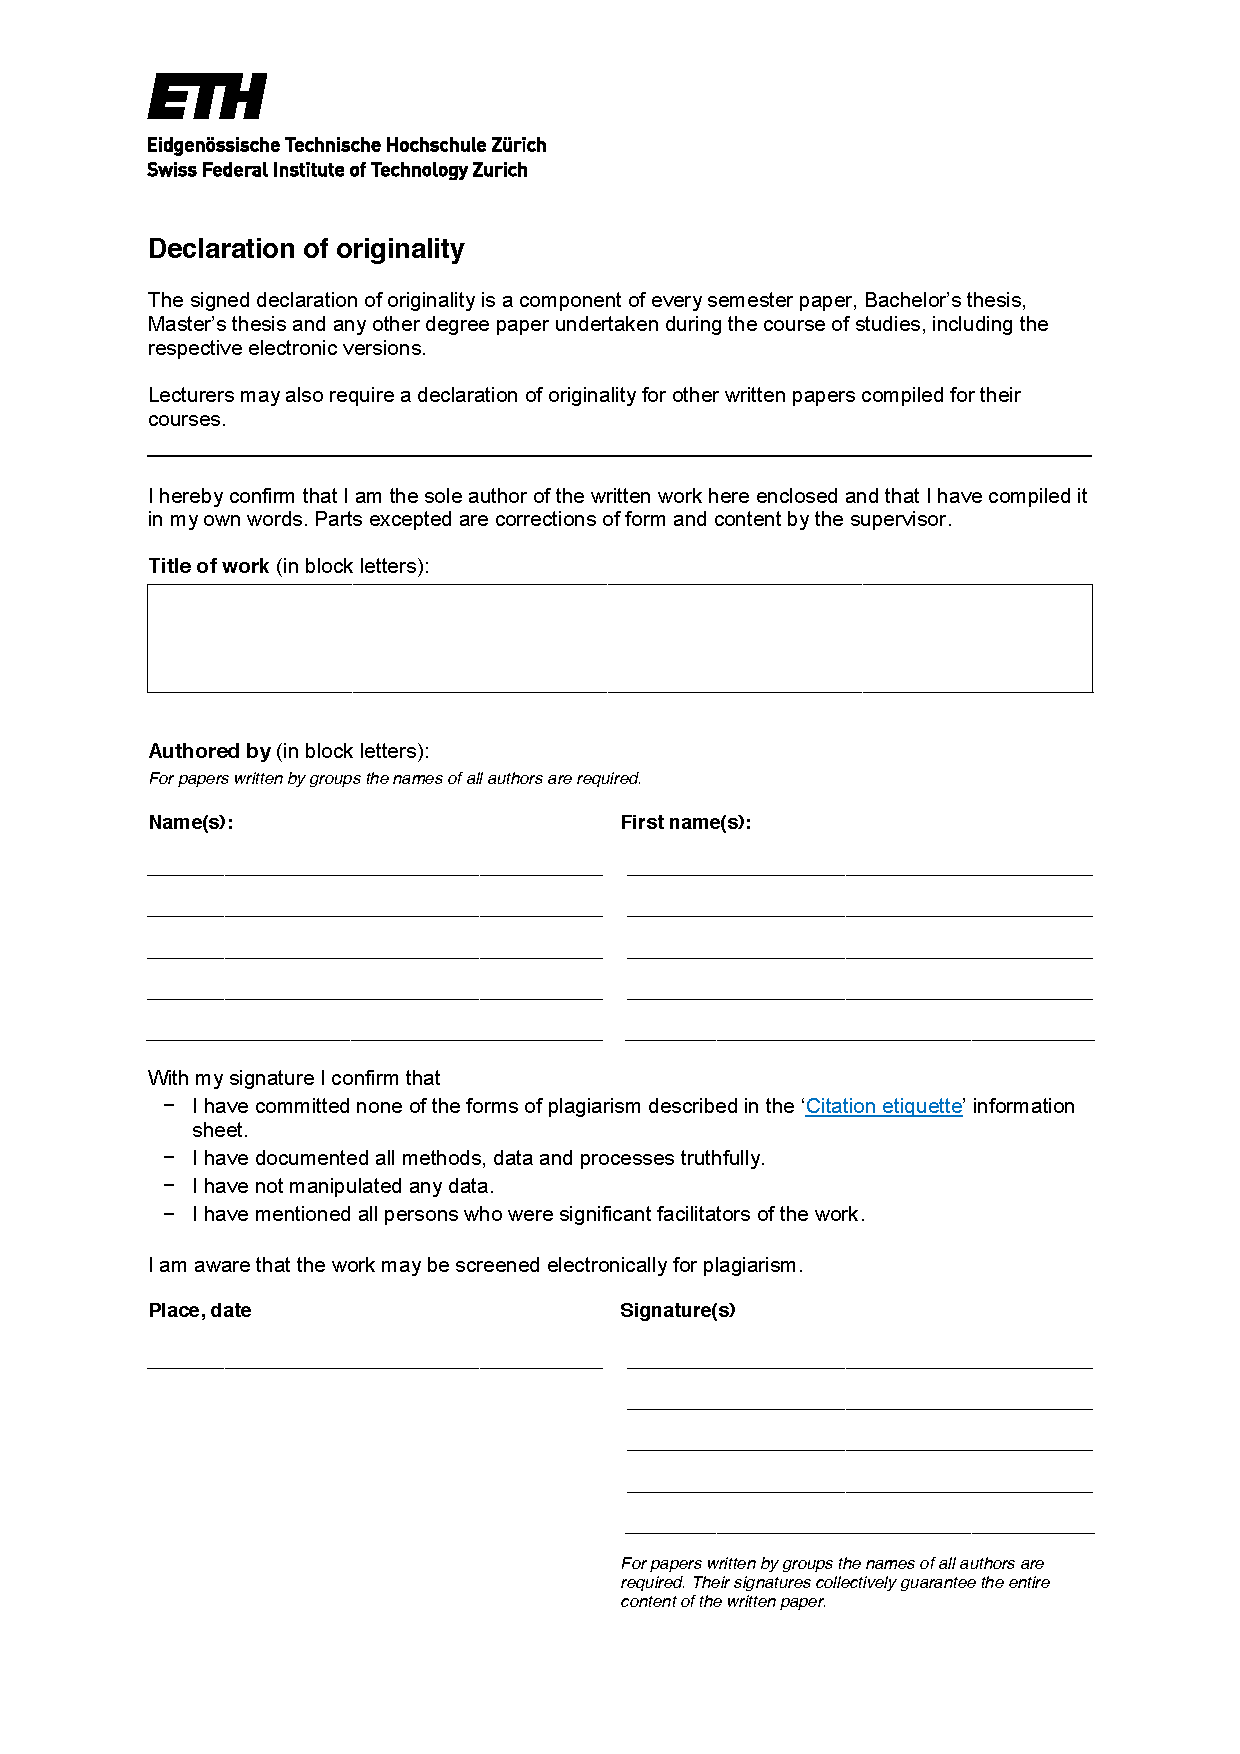
\includepdf[pages={-}]{declaration-originality.pdf}

\end{document}
